\documentclass{senior-design}

%%% Watermark %%%%%%%%%%%%%%%%%%%%%%%%%%%%%%%%%%%%%%%%%%%%%%%%%%%
\usepackage[scale=1,
            % final, % uncomment this line to disable the watermark
            text=SAMPLE]{draftwatermark}

%%% Fonts %%%%%%%%%%%%%%%%%%%%%%%%%%%%%%%%%%%%%%%%%%%%%%%%%%%%%%%
\setmonofont[Scale=MatchLowercase]{Consolas}
\setsansfont{Arial}
\usepackage{newpxtext, newpxmath} % Palatino

%%% Report information %%%%%%%%%%%%%%%%%%%%%%%%%%%%%%%%%%%%%%%%%%
\reporttitle{An Awesome Project Made By An Amazing Team}
\reporttype{Final Report} % Uncomment this line if you want to use \generalreportcover
\semester{Spring 2023}
\sponsor{Prof. \name{Sansan}{Zhang}}
\ta{\name{Sisi}{Li}}
\reportdate{\today}
\authornames{
    \nameemail{San}{Zhang}{sanz0@illinois.edu}\\[1em]
    \nameemail{Si}{Li}{sil0@illinois.edu}\\[1em]
    \nameemail{Dawu}{Wang}{dawu@example.com}\\[1em]
    \nameemail{English}{Member}{englishm0@illinois.edu}
}
\addbibresource{references.bib} % The bib database
%%%%%%%%%%%%%%%%%%%%%%%%%%%%%%%%%%%%%%%%%%%%%%%%%%%%%%%%%%%%%%%%%

%%% Uncomment the lines you need according to the type of report:
\projectnumber{114}
\teamnumber{514}
%%%%%%%%%%%%%%%%%%%%%%%%%%%%%%%%%%%%%%%%%%%%%%%%%%%%%%%%%%%%%%%%%

\begin{document}
%%% TITLE PAGE: select the one you need %%%%%%%%%%%%%%%%%%%%%%%%%
\generalreportcover % coverpage for other reports; NEEDS \reporttype{<Type>}
%%%%%%%%%%%%%%%%%%%%%%%%%%%%%%%%%%%%%%%%%%%%%%%%%%%%%%%%%%%%%%%%%
\frontmatter

%%% Acknowledgement %%%%%%%%%%%%%%%%%%%%%%%%%%%%%%%%%%%%%%%%%%%%%
\chapter*{Acknowledgement}\thispagestyle{acknowledgement}
Writing an acknowledgment section is a way to express your gratitude to individuals and organizations that have contributed to your project. Below are some tips on how to write an acknowledgment section:

Begin your acknowledgment section by expressing your gratitude to the individuals or organizations that have helped you with your project. This can include your faculty advisor, project sponsor, team members, family members, and friends.

Be specific about the contributions that each person or organization has made to your project. This can include providing technical guidance, financial support, or emotional support.
It's important to keep your acknowledgment section concise. Try to limit your acknowledgments to one page or less.
Keep in mind that your acknowledgment section is part of a formal report, so please use a professional tone and avoid overly casual language.

%%%%%%%%%%%%%%%%%%%%%%%%%%%%%%%%%%%%%%%%%%%%%%%%%%%%%%%%%%%%%%%%%

%%% Abstract %%%%%%%%%%%%%%%%%%%%%%%%%%%%%%%%%%%%%%%%%%%%%%%%%%%%
\chapter*{Abstract}\thispagestyle{abstract}
The abstract is short (150 words or less) and provides enough of a summary of the report for the reader to decide whether to read the entire document. State very concisely what your device or system does, and the main findings and results of your project. Save background information (e.g., motivation, competitors) for the introduction and design details for the body of the report. Do not give an advertising pitch. Note that the abstract does not appear in the table of contents. (This is achieved by using \verb|\chapter*| command instead of \verb|\chapter|.)

Note that you can ignore the TOC because it is generated automatically by \verb|\tableofcontents| below. Work on the body of the report, then compile the project using the following commands:
\begin{lstlisting}
xelatex sample_general.tex
biber sample_general
xelatex sample_general.tex
xelatex sample_general.tex
\end{lstlisting}

\paragraph{Keywords}
% Put keywords below
Keyword 1, keyword 2, keyword 3
%%%%%%%%%%%%%%%%%%%%%%%%%%%%%%%%%%%%%%%%%%%%%%%%%%%%%%%%%%%%%%%%%

%%% TOC %%%%%%%%%%%%%%%%%%%%%%%%%%%%%%%%%%%%%%%%%%%%%%%%%%%%%%%%%
\tableofcontents\thispagestyle{toc}
%%%%%%%%%%%%%%%%%%%%%%%%%%%%%%%%%%%%%%%%%%%%%%%%%%%%%%%%%%%%%%%%%

\mainmatter
%%% Body %%%%%%%%%%%%%%%%%%%%%%%%%%%%%%%%%%%%%%%%%%%%%%%%%%%%%%%%
\chapter{Introduction}
Briefly describe the science or engineering problem to be addressed in the report, as well as the purpose and usefulness of the device or system you have built. Summarize the contents of the upcoming chapters as well as the main conclusions of your project, to be elaborated in the last chapter.

\section{Sample citation using IEEE}
Here comes the citation. You can cite by using \verb|\cite| which produces \cite{book1,paper1}, or by \verb|\textcite| which produces \textcite{book2}. However, putting a citation at the end of a sentence is also acceptable \cite{webpage1}.

\section{Sample equations}
\begin{equation}
    EQI = \sum_{i=1}^{n}W_j * r_{ij}
\end{equation}

\begin{equation}
    EHI = L_1 \times ESI + L_2 \times EQI
\end{equation}

\begin{equation}
    \begin{aligned}
        EE / EHI = \beta_0 & + \beta_1 PCG + \beta_2 RGP + \cdots + \beta_i X_i +              \\
        \cdots             & + \beta_9 ICWUR + \beta_{10} ECPG + \beta_11 WCPG + \varepsilon_i
    \end{aligned}
\end{equation}

\section{Sample listings}
This is a sample listing.
\begin{lstlisting}[language=c]
#include<stdio.h>
void fuzzy(int x){
    return x;
}
int main(){
    int a = 0, b, c;
    scanf("%d", &b);
    c = b;
    if (a == b)
        a = fuzzy(c);
    else
        b = fuzzy(a);
    printf("%d %d\n", a, fuzzy(c));
    return 0;
}
\end{lstlisting}

\chapter{Design}
Discuss general design alternatives. Give equations, simulations, and general circuits. Describe the design in detail, addressing each major component. Include schematics with components, drawings, flowcharts, etc. Some teams may wish to split this chapter in two: 2. Design Procedure, and 3. Design Details. This \LaTeX~template will automatically update numbering systems for chapters, sections, figures, tables, etc., yet you should still always keep track of them as you develop and revise the text.

\section{Typesetting SI Units}
This template allows you to typeset SI units in a standard format. The units should be typed like this: \SI{10e5}{\um\ohm\degree}.

It also applies to equations,
\begin{equation}
    X_{t}=\SI{10e5}{\um\ohm\degree}
\end{equation}

Visit \url{https://www.ctan.org/pkg/siunitx} for more details about package \texttt{siunitx}.

\chapter{Design Verification}
\begin{figure}[H]
    \centering
    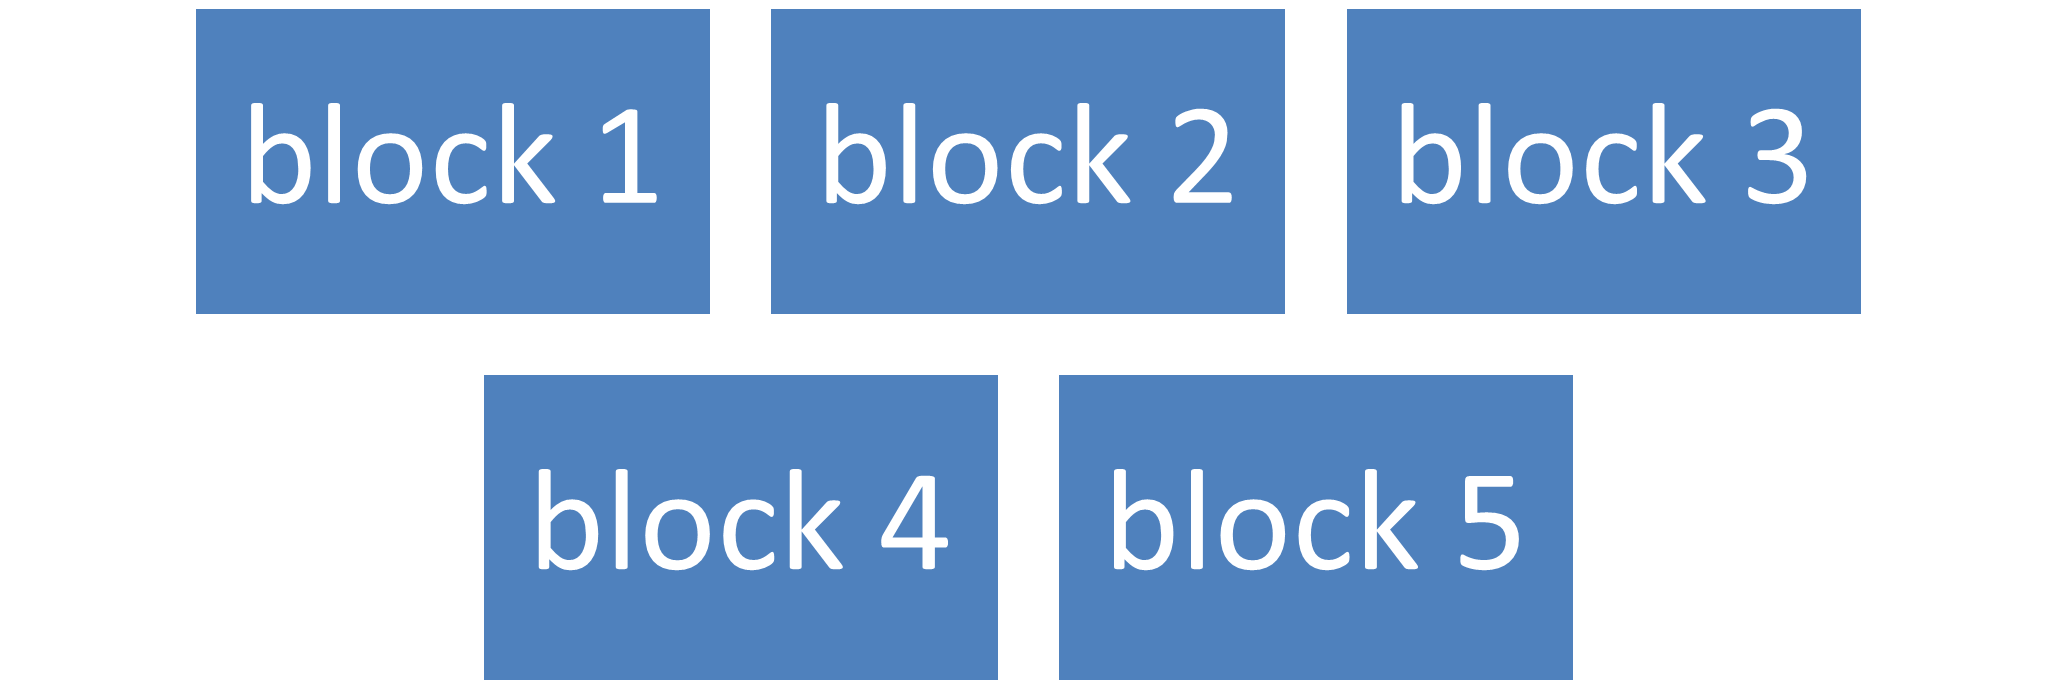
\includegraphics[width=0.8\linewidth]{figs/Picture1.png}
    \caption{An example figure.}
\end{figure}

\chapter{Discussion}

\section{A sample of table}
\begin{table}[H]
    \centering
    \caption{Example of a Table and Its Title}
    \label{tab:eg-table}
    \begin{tabular}{@{}c|cc@{}}
        \toprule
        Part                & Electricity  & Magnetism \\ \midrule
        Field intensity     & $E$          & $H$       \\
        Flux density        & $D$          & $B$       \\
        Constitutive factor & $\epsilon^b$ & $\mu$     \\ \bottomrule
    \end{tabular}
\end{table}

\section{An example of inserting code listings}
An example piece of inserting code from an existing file:
\lstinputlisting[language=python]{code/example.py}

\chapter{Conclusion}

\begin{equation}
    F\left( x \right) =\begin{cases}
        0,&		x<a\\
        \frac{x-a}{b-1},&		a\leqslant x<b\\
        1,&		x\geqslant b\\
    \end{cases}
\end{equation}

\section{Accomplishments}
\section{Uncertainties}
\section{Ethical Considerations}
\section{Future Work}
%%%%%%%%%%%%%%%%%%%%%%%%%%%%%%%%%%%%%%%%%%%%%%%%%%%%%%%%%%%%%%%%%

%%% References %%%%%%%%%%%%%%%%%%%%%%%%%%%%%%%%%%%%%%%%%%%%%%%%%%
\clearpage
\renewcommand*{\UrlFont}{\rmfamily}
\printbibliography[title={References},heading=bibintoc]
\thispagestyle{references}
\clearpage
%%%%%%%%%%%%%%%%%%%%%%%%%%%%%%%%%%%%%%%%%%%%%%%%%%%%%%%%%%%%%%%%%

%%% Appendices %%%%%%%%%%%%%%%%%%%%%%%%%%%%%%%%%%%%%%%%%%%%%%%%%%
\begin{appendices}
    % All appendices here, using sections for multiple appendices
    \chapter{Requirement and Verification Table}
    An appendix is a good place for the Requirement and Verification Table from your design review. Below is a starter table. Including these details here will help to avoid lengthy and tedious narrative descriptions in the main text, which may not be of immediate interest to your imagined audience of company managers and professionals. Any requirement that is not verified should be explained either in the main text or the appendix. Note that both the pagination and the numbering of figures, tables, and equations continue from the main text to the appendices.

    Tab. \ref{tab:srv} is generated by Excel2LaTeX. See \url{https://www.ctan.org/tex-archive/support/excel2latex/} for more details.
    % Table generated by Excel2LaTeX from sheet 'Sheet1'
    \begin{table}[htbp]
        \centering
        \caption{System Requirements and Verifications}
        \begin{tabularx}{\textwidth}{X|X|c}
            \toprule
            \centering\multirow{2}[2]{*}{Requirement} & \centering\multirow{2}[2]{*}{Verification} & \multicolumn{1}{c}{Verification status} \\
            \multicolumn{1}{c|}{}                     & \multicolumn{1}{c|}{}                      & \multicolumn{1}{c}{(Y or N)}                     \\
            \midrule
            1. Requirement                            & 1. Verification                            & \multirow{4}[1]{*}{}                             \\
            a. Subrequirement                         & a. Subverification                         &                                                  \\
            b. Subrequirement                         & b. Subverification                         &                                                  \\
            c. Subrequirement                         & c. Subverification                         &                                                  \\\hline
            2. Requirement                            & 2. Verification                            & \multirow{4}[0]{*}{}                             \\
            a. Subrequirement                         & a. Subverification                         &                                                  \\
            b. Subrequirement                         & b. Subverification                         &                                                  \\
            c. Subrequirement                         & c. Subverification                         &                                                  \\\hline
            3.                                        & 3.                                         &                                                  \\\hline
            4.                                        & 4.                                         &                                                  \\\bottomrule
        \end{tabularx}%
        \label{tab:srv}%
    \end{table}%

    \section{Some Test Data}
\end{appendices}
\clearpage
%%%%%%%%%%%%%%%%%%%%%%%%%%%%%%%%%%%%%%%%%%%%%%%%%%%%%%%%%%%%%%%%%
\backmatter
\end{document}